%!TEX root = main.tex
\chapter{TRIAC en tryristor}
\label{TRIAC_en_tryristor}

\section{Tryristor}
Een tryristor heeft de volgende schakeling:
%thyristor schakeling
\begin{center}
    \begin{circuitikz}
        \draw (0,0) to [isourcesin](0,2)
        to [Ty, n=Tro](2,2)
        to [european resistor](2,0)
        to [short](0,0);
    \end{circuitikz}
\end{center}

Met het symbool $\alpha$ wordt de stuurhoek aangegeven. Dit is de hoek waar het signaal bij begint. het signaal voor deze hoek is
afgekapt en dus afwezig. Dit wordt elke $2\pi$ herhaald. Het stuk tussen 0 graden een de stuurhoek is dus altijd 0. Dit  is goed 
te zien in \cref{fig:thyristor_spanning}.

\begin{figure}
    \begin{center}
    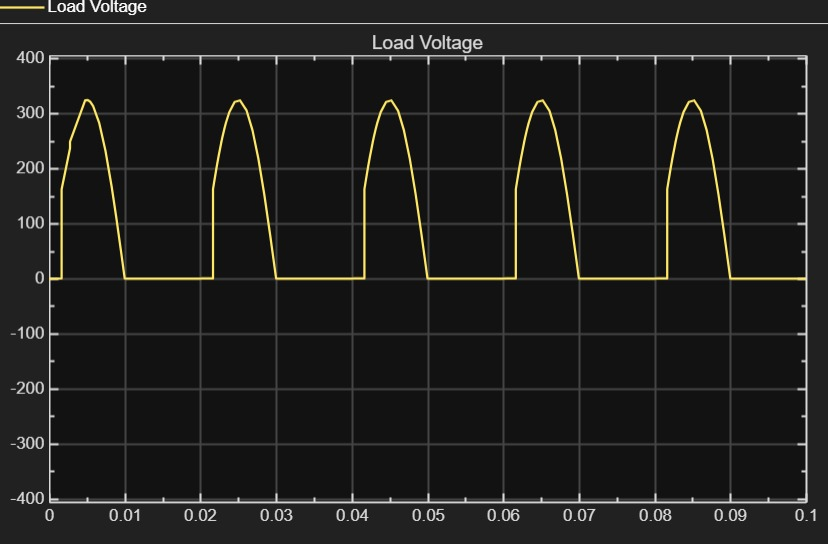
\includegraphics[width=0.5\linewidth]{afbeeldingen/IMG-20260316-WA0006.jpg}
    \caption{Spanning over de weerstand bij een thyristor}
    \label{fig:thyristor_spanning}
    \end{center}
\end{figure}

Over $U_R$ staat ook deze spanning. De spanning is echter alleen positief. De negative spanningen zijn over de weerstand 0v.

Bij het rekenen aan de schakeling horen de volgende formules:

$U_{Rrms}=\frac{\hat{u}}{2}\sqrt{\frac{\pi -\alpha }{\pi }+\frac{\sin (2\alpha )}{2\pi }}$

$U_{1rms}=\frac{\sqrt{a_1^2 + b_1^2}}{2\pi }$

$a_1=\frac{\hat{u}}{2 \pi} \left(\pi - \alpha + \frac{\sin (2 \alpha)}{2}\right) $

$b_1=\frac{\hat{u}}{2 \pi} \left(\frac{\cos (2 \alpha)}{2} \right) $

$S_1=U_b \cdot I_1$

$I_1=\frac{U_b}{R}$

\vspace{5mm}

De rest van de formules zijn makkelijk te achter halen met behulp van de vermogens driehoek. Deze kan voor de berekeningen van de 
tryristor en de TRIAC worden uitgebreid. Dit komt er dan als volgende uit te zien:
%vermogens driehoek uitgebrijdt
\begin{center}

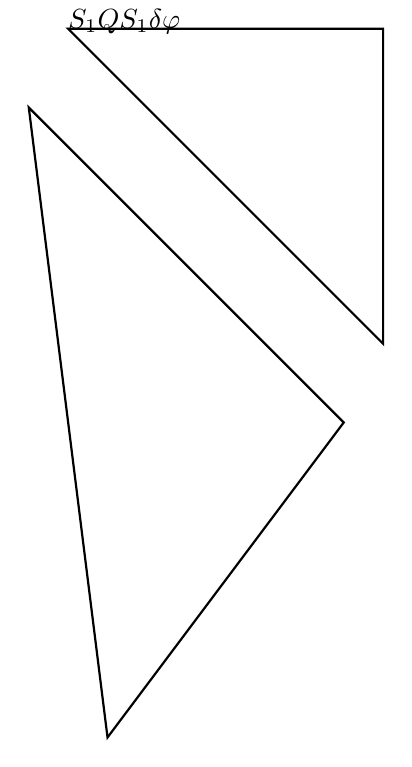
\begin{tikzpicture}[thick]
\coordinate (O) at (0,0);
\coordinate (A) at (4,0);
\coordinate (B) at (4,-4);
\draw (O)--(A)--(B)--cycle;

\coordinate (x) at (3.5,-5);
\coordinate (y) at (-0.5,-1);
\coordinate (z) at (0.5,-9);
\draw (x)--(y)--(z)--cycle;

\tkzLabelSegment[above=2pt](O,A){\textit{P}}
\tkzLabelSegment[left=2pt](O,B){\textit{$S_1$}}
\tkzLabelSegment[above right=0pt](A,B){\textit{$Q$}}

\tkzLabelSegment[left=2pt](y,z){\textit{S}}
\tkzLabelSegment[left=2pt](x,y){\textit{$S_1$}}
\tkzLabelSegment[below=2pt](x,z){\textit{D}}

\tkzMarkAngle[fill= teal,size=0.8cm,%
opacity=.4](B,O,A)
\tkzLabelAngle[pos = -0.6](A,O,B){$\delta $}

\tkzMarkAngle[fill= teal,size=0.8cm,%
opacity=.4](z,y,x)
\tkzLabelAngle[pos = -0.6](x,y,z){$\varphi $}

\end{tikzpicture}
\end{center}

binnen de driehoek geldt: 

$S_1=$ Eerste harmonische van S

$S=$ Totaal vermogen.

$D=$ Distortie vermogen.

Tijdens het lab zijn er metingen gedaan aan een thyristor. In \cref{tab:thyristor}
is goed te zien wat het effect is van de stuurhoek op zowel de RMS waarde van de spanning als op het vermogen.
\footnote{De bij de metingen in \cref{tab:thyristor} mocht de spanning veel hoger. Dit was wegens eigen veiligheid en limiten 
op de aparatuur niet mogelijk.}

\begin{table}
    \begin{center}
    \begin{tabular}{|c|c|c|c|}
        \arrayrulecolor{purple}\hline
	    \rowcolor{purple} 
	    \multicolumn{1}{c}{\textcolor{white}{\textbf{$\alpha$}}} & \multicolumn{1}{c}{\textcolor{white}{\textbf{$U_{load}(mV)$}}} &
        \multicolumn{1}{c}{\textcolor{white}{\textbf{$I_{load}(mA)$}}} & \multicolumn{1}{c}{\textcolor{white}{\textbf{$P_{load}(W)$}}} 
        \\ \hline
            $30^\circ$ & 768 & 6.65 & $5.107\cdot 10^{-2}$ 
            \\ \hline
            $60^\circ$ & 692 & 6.73 & $4.657\cdot 10^{-2}$ 
            \\ \hline
            $90^\circ$ & 473 & 5.87 & $2.776\cdot 10^{-2}$ 
            \\ \hline
    \end{tabular}
    \caption{Metingen thyristor lab}
    \label{tab:thyristor}
    \end{center}
\end{table}

\section{TRIAC}
Een TRIAC heeft net een andere, maar vergelijkbare schakeling:
%TRIAC schakeling
\begin{center}
    \begin{circuitikz}
        \draw (0,0) to [isourcesin](0,2)
        to [Tr, n=Tyo](2,2)
        to [european resistor](2,0)
        to [short](0,0);
    \end{circuitikz}
\end{center}

Voor de TRIAC gelden de zelfde formules er, maar omdat de schakeling anders is zijn er wel 3 formules verandert:

$U_{Rrms}=\frac{\hat{u}}{\sqrt{2}}\sqrt{\frac{\pi -\alpha }{\pi }+\frac{\sin (2\alpha )}{2\pi }}$

$a_1=2\frac{\hat{u}}{2 \pi} \left(\pi - \alpha + \frac{\sin (2 \alpha)}{2}\right) $

$b_1=2\frac{\hat{u}}{2 \pi} \left(\frac{\cos (2 \alpha)}{2} \right)$

De TRIAC is in principe een dubbele thyristor. Hier door komt de spanning over de weerstand er andes uit te zien zie
\cref{fig:triac_spanning}

\begin{figure}
    \begin{center}
    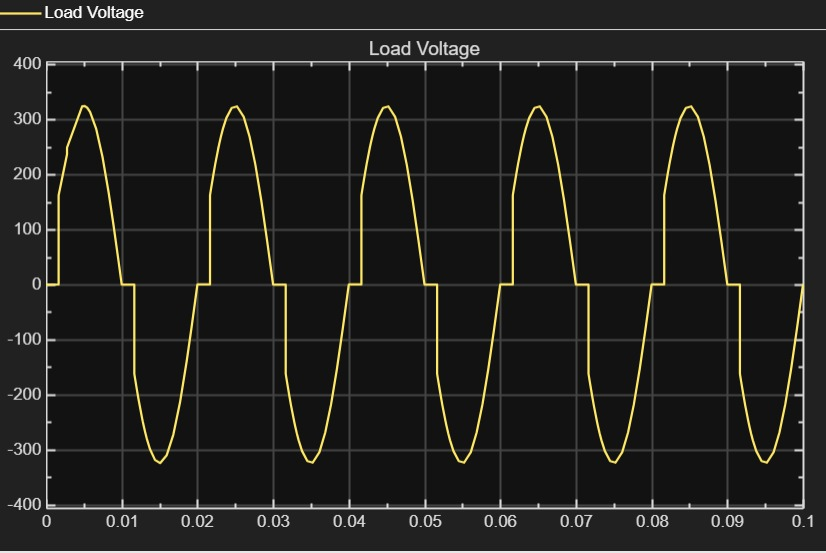
\includegraphics[width=0.5\linewidth]{afbeeldingen/IMG-20260316-WA0011.jpg}
    \caption{Spanning over de weerstand bij een TRIAC}
    \label{fig:triac_spanning}
    \end{center}
\end{figure}

Tijden het lab is gewerkt met een TRIAC. De metingen zijn te vinden in \cref{tab:triac}
In de tabel is een duidelijk verschil te zien tussen de RMS waarden van de spanning en de vermogens bij de TRIAC en de thyristor 
\cref{tab:thyristor}.
\footnotetext{In de test van \cref{tab:triac} was wegens een verwacht hoger vermogen een andere load gebruikt. De waardes zijn
dus niet perfect te vergelijken, maar geven wel een goed inzicht wat er gebeurt. Daarnaast is de load alleen veranderd omdat 
er een hoger vermogen werd verwacht.}
\footnote{De spanning is bij de metingen van \cref{tab:triac} naar het maxium van 30V aangepast.}

\begin{table}
    \begin{center} 
    \begin{tabular}{|c|c|c|c|}
        \arrayrulecolor{purple}\hline
	    \rowcolor{purple} 
	    \multicolumn{1}{c}{\textcolor{white}{\textbf{$\alpha$}}} & \multicolumn{1}{c}{\textcolor{white}{\textbf{$U_{load}(V)$}}} &
        \multicolumn{1}{c}{\textcolor{white}{\textbf{$I_{load}(mA)$}}} & \multicolumn{1}{c}{\textcolor{white}{\textbf{$P_{load}(W)$}}} 
        \\ \hline
            $30^\circ$ & 32.44 & 102.0 & 3.33 
            \\ \hline
            $60^\circ$ & 30.16 & 88.7 & 2.88
            \\ \hline
            $90^\circ$ & 23.3 & 62.9 & 1.73
            \\ \hline
    \end{tabular}
    \caption{Metingen TRIAC lab}
    \label{tab:triac}
    \end{center}
\end{table}